\section{Kapacitet}
% Skriv ift kapacitet (ift sengepladser, persona - hvilken betydning har hhv. 95 \% kapacitet mod 105 \%)
Kapacitet omfatter antallet af patienter, kontakter, personale, udstyr og rum. Kontrakter omfatter forundersøgelse, behandling og kontrol. Personalet består af læger, sygeplejersker og sekretærer. Udstyret beskriver de nødvendige maskiner samt antallet af rum der er udstyret med disse. Dette beskriver den samlede kapacitetsudnyttelse som defineres som  mest mulig producering af investerede ressourcer og er forholdet mellem aktivitet og kapacitet. \cite{Company2013} En beskrivelse af dette fremgår af \figref{kapacitet}. 

\begin{figure}[H]
	\flushleft 
	\centering
	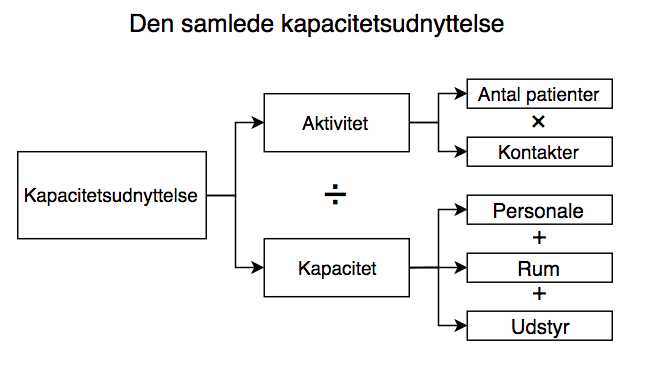
\includegraphics[scale=.45]{figures/Kapacitetsudnyttelse.png}
	\label{kapacitet}
	\flushleft
	\textit{Flowdiagramet viser den samlede kapacitetsudnyttelse som er inddelt i aktivitet og kapacitet \cite{Company2013}}
\end{figure}


%Definition af kapacitet er maksimal ydeevne for en afdeling og benyttes som et mål for, hvordan denne udnyttes i en bestemt sammenhæng f.eks. i forbindelse med et belægningsproblem.
\noindent

Belægning beskriver antallet af patienter, der er normeret til på en afdeling \cite{Heidmann2014}. Når en $100~\%$ belægning opnås svarer dette til at alle sengepladser på en afdeling er taget i brug hvilket er fuld udnyttelse af kapaciteten. Ved en belægningsgrad på over $100~\%$ betyder det, at der er flere patienter end afdelingen er normeret til, hvilket vil sige, at afdelingen yder mere end der er kapacitet til. Ved en belægningsgrad på under $100~\%$ er der omvendt færre patienter end afdelingen er normeret til, således der er tomme sengepladser og afdelingen derved ikke udnytter kapaciteten effektivt. \cite{Pauly1986} 

\subsection{Ortopædkirurgisk afdeling}
Ortopædkirurgisk afdeling udgør $4~\%$ af det samlede antal ydelser for de forskellige afdelinger på Aalborg Universitetshospital. Derudover udgør fordelingen af nordjydernes anvendelse af ortopædkirurgisk afdeling $5,6\%$ af det samlede forbrug til de forskellige afdelinger. Dette svarer til et bruttohonorar på $13.550.874,38$~kr. \cite{RegionNord2016}. Ortopædkirurgik afdelingen varetager behandlingen af skader på knogler, muskler, sener eller led og består af 10 fagområder. Fagområderne omfatter: Børneortopædkirurgi, knogle- og rekonstruktion, fod- og ankelkirurgi, knæ- og hoftekirurgi, håndkirurgi, ryg- og bækkenkirurgi, knæ- og idrætsskader, tumor- og sarkomkirurgi, amputationer og sår, samt traumatologi. Afdelingen er delt op i 5 afsnit bestående af sengeafsnit O1 og O2 på 5. sal, operationsafsnit på 1. sal, sammedagskirurgi afsnit O6, samt ambulatorium. \cite{Aalborg2016}


\subsubsection{Udnyttelse af personale - MANGLER VIDEN} 
% Hvordan opleves belægning generelt på OA på AUH? Hvordan varetages opgaver af personalet? Hvordan er vagtskifte? Hvor langt tid arbejdes der gennemsnitlig om dagen?
Sundhedspersonalet på ortopædkirurgisk afdeling på Aalborg Universitetshospital arbejder i gennemsnit 37 timer om ugen, hvilket svarer til XX antal timer om dagen. \cite{Danske2015} Under normale omstændigheder varetager sundhedspersonalet XX antal patienter fordelt på XX timer. Afdelingen er delt op i XX antal vagthold og har vagtskifte hver XX time. Personalets opgaver varetages på følgende måder XX.x

\subsubsection{Indlæggelse af personale - MANGLER VIDEN}
% Hvordan foregår indlæggelsen på OA på AUH? Hvornår indlæggelses patienterne (elektive patienter) og hvornår på dagen udskrives patienter (både elektive og akutte patienter) Hvor mange patienter hhv. akutte vs. elektive patienter? Hvad er deres buffer i forhold til elektive patienter, således der er plads til de akutte indlæggelser? indkaldes elektive patienter, hvis der er mindre akutte i en periode end der er estimeret til? Øges den normerede kapacitet under overbelægning ved at indkalde vikarbureau? (Altså tager man samme mængde elektive patienter ind.) 
Afdelingen har sengepladser til XX patienter til rådighed. En stigning i ambulante besøg på Aalborg Universitetshospital fra år $2010$ til $2013$ har medført at sengedagene på hospitalet har været faldende på grund af omlægningen fra stationær aktivitet til ambulant. Dette betyder et fald i sengedage på $6~\%$ for akutte og $19~\%$ for elektive patienter. Andelen af akutte indlæggelser i Region Nordjylland udgør $76~\%$, hvor de resterende $24~\%$ er elektive.\fxnote{er det kun for ortopæd?} \cite{RegionNord2016}. Hvis der ses på ortopædkirurgisk afdeling svarer dette til XX antal akutte og XX antal elektive patienter. Hvis der sammenlignes med andre afdelinger på Aalborg Universitetshospital er ortopædkirurgisk afdeling den afdeling der har flest elektive indlæggelser, hvilket svarer til $13~\%$ af de samlede indlæggelser. \cite{RegionNord2016}. Elektive patienter indlægges XX på dagen og udskrives igen XX på dagen. Derudover har sundhedspersonalet en 'buffer' i forhold til elektive patienter på XX antal dage for, at gøre plads til akutte indlæggelser. Elektive patienter kan derudover tilkaldes hvis antallet af akutte indlæggelser falder over en periode. 

\begin{figure}[H]
	\flushleft 
	\centering
	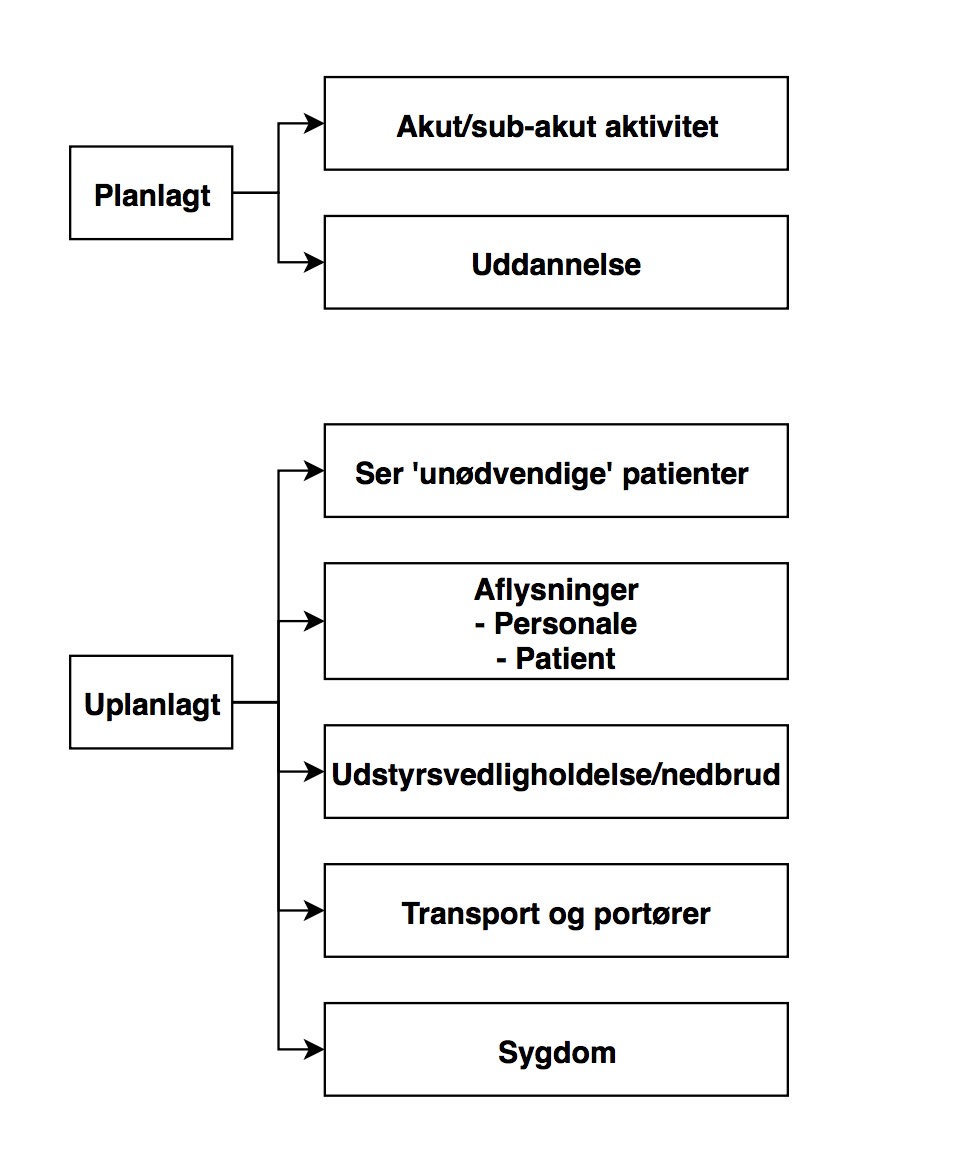
\includegraphics[scale=.45]{figures/planlagtakutte.png}
	\label{planlagtakutte}
	\flushleft
	\textit{Flowdiagramet viser fordelingen af elektive og akutte patienter\cite{Company2013}}
\end{figure}